\section{Implementation}

A prototype tool was developed on top of the Solidity compiler to allow the application of our technique. Given a Solidity contract, the prototype automatically generates the constrained Horn clauses representing it, which can then be supplied to off-the-shelf Horn clause solvers.

The clause generation is integrated in the compilation process and has two steps. First, the prototype traverses the AST of the contract and constructs the control flow graph representing it. The second step is to generate the constrained Horn clauses from the control flow graph constructed. The CFG is a suitable intermediate structure that can be easily constructed from the AST and that allows for a direct mapping into Horn clauses; for ease of implementation we construct a single graph for the whole contract in the first step, instead of combining in the second step the clauses generated from the graphs of each function.

For each function in the contract, including the constructor, the prototype creates a local control flow graph, and then it integrates all of them in a single graph in order to model the contract behaviour on the blockchain. Each local control flow graph has an entry and exit block. From the entry block, every time a control structure, such as a conditional or a loop, is reached, the graph is updated with new blocks; the position of the edges, and thus the topology of the graph, depend on the semantics of each control structure in the function.

Statements in the body of a function that do not influence its control flow, such as assignments and \texttt{require} statements, are associated with a block in the graph according to their position in the code, modelling $\lambda$. A block $b$ that exists only for control purposes, with no associated statements, $\lambda(b) = true$, is called an empty block.

To model the contract graph, three new empty blocks are created: global entry, interface, and error. The global entry represents the start of the contract models a call to the constructor. The interface allows calls to the contract functions in nondeterministic order; its outward edges target the entry block of each function and its inward edges depart from the exit block each function. A single error block is modelled at the contract level, being targeted by by all failed assertions in the code, instead of individual error blocks for each function. The control flow graph constructed for the contract in Figure \ref{fig:contractC} can be seen in Figure \ref{fig:cfg_contract-c}; the \texttt{\#} stands for a nondeterministic assignment to the function arguments. 

\begin{figure}[h]
	\centering
	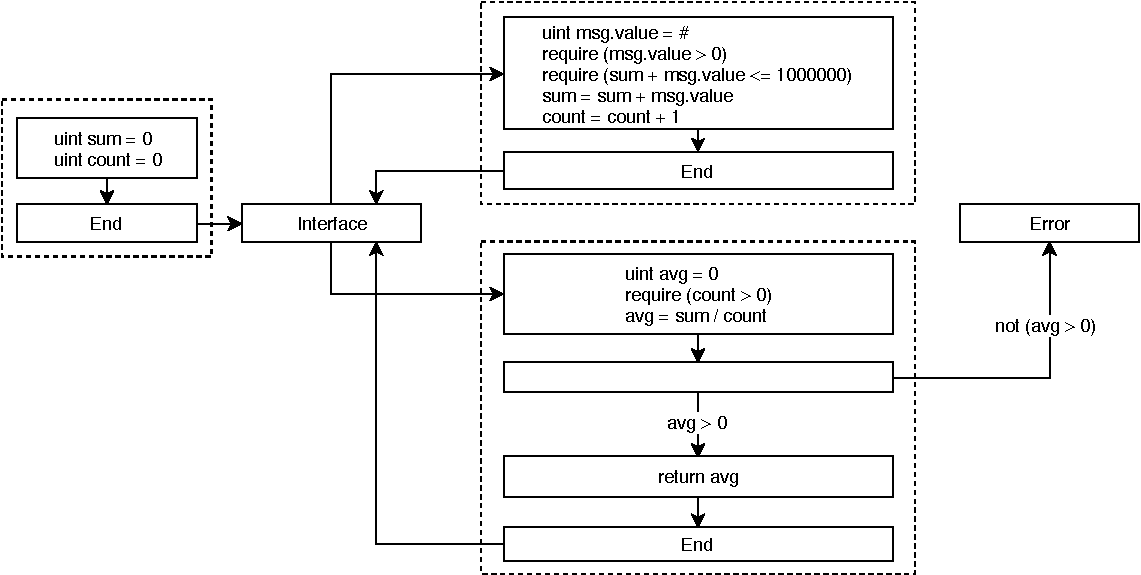
\includegraphics[width=0.49\textwidth]{images/contract-c}
	\caption{Control flow graph modelling the \texttt{C} contract}
	\label{fig:cfg_contract-c}
\end{figure}

From the control flow graph of the contract, the constrained  Horn clauses can be directly extracted. The transition from the entry block to the constructor, and from the constructor to the interface block, are modelled as Eq. \ref{eq:CHC-constructor-initial} and Eq. \ref{eq:CHC-constructor-final}. The interaction between the interface and the functions is modelled as Eq. \ref{eq:CHC-call-initial} and Eq. \ref{eq:CHC-call-final}. For the functions themselves, entry and exit blocks are modelled as Eq. \ref{eq:CHC-initial} and Eq. \ref{eq:CHC-final}, and their bodies are modelled according to Eq. \ref{eq:CHC-transition}; the prototype does not implement $\rho$, using the state variables directly instead of creating temporary local variables to represent them, this change avoids the overhead of having local copies and does not affect the soundness of the implementation.

The prototype currently implements the generation of Horn clauses for a subset of the Solidity language. Most basic arithmetic and control flow operators, as well as assertions, are supported. Regarding data, the prototype fully supports integer variables and has partial support for arrays. Function calls, recursive or otherwise, additional value and reference types, such as strings and structs, are not yet supported; the limitations are specific to the prototype, and are not present in the formal modelling.

% Early versions

%The CFG of a given Solidity contract is constructed by first defining global entry and error blocks, together with the interface block. The entry block represents the start of the contract and models a call to the constructor, Eq. \ref{eq:CHC-constructor-initial}. The interface block allows calls to the contract functions in nondeterministic order, directly modelling the $\conP(\svar)$ predicate; its outward and inward edges model Eq. \ref{eq:CHC-call-initial} and Eq. \ref{eq:CHC-call-final}, respectively. Instead of local error states for each function, the prototype creates a single global error state for the whole contract.

%Given a current node $m \in V$, the occurrence of a while loop, for example, leads to the creation of four new nodes $loop1, loop2, loop3, n \in V$, with $loop1$ capturing the loop condition, $loop2$ and $loop3$ modelling the start the end of its body, and $n$ being the first block after the loop. The edge $\langle m, loop1 \rangle$ models the start of the loop, $\mu(\langle m, loop1 \rangle) = true$, the edge $\langle loop1, loop2 \rangle$ models the start of the body of the loop, $\mu(\langle m, loop1 \rangle) = condition$, the edge $\langle loop2, loop3 \rangle$ models the end of the body of the loop, $\mu(\langle loop3, loop1 \rangle) = true$, and the edge $\langle loop3, m \rangle$ models the exit of the loop $\mu(\langle m, loop1 \rangle) = \neg condition$.